\documentclass{article}\usepackage[]{graphicx}\usepackage[]{color}
%% maxwidth is the original width if it is less than linewidth
%% otherwise use linewidth (to make sure the graphics do not exceed the margin)
\makeatletter
\def\maxwidth{ %
  \ifdim\Gin@nat@width>\linewidth
    \linewidth
  \else
    \Gin@nat@width
  \fi
}
\makeatother

\definecolor{fgcolor}{rgb}{0.345, 0.345, 0.345}
\newcommand{\hlnum}[1]{\textcolor[rgb]{0.686,0.059,0.569}{#1}}%
\newcommand{\hlstr}[1]{\textcolor[rgb]{0.192,0.494,0.8}{#1}}%
\newcommand{\hlcom}[1]{\textcolor[rgb]{0.678,0.584,0.686}{\textit{#1}}}%
\newcommand{\hlopt}[1]{\textcolor[rgb]{0,0,0}{#1}}%
\newcommand{\hlstd}[1]{\textcolor[rgb]{0.345,0.345,0.345}{#1}}%
\newcommand{\hlkwa}[1]{\textcolor[rgb]{0.161,0.373,0.58}{\textbf{#1}}}%
\newcommand{\hlkwb}[1]{\textcolor[rgb]{0.69,0.353,0.396}{#1}}%
\newcommand{\hlkwc}[1]{\textcolor[rgb]{0.333,0.667,0.333}{#1}}%
\newcommand{\hlkwd}[1]{\textcolor[rgb]{0.737,0.353,0.396}{\textbf{#1}}}%

\usepackage{framed}
\makeatletter
\newenvironment{kframe}{%
 \def\at@end@of@kframe{}%
 \ifinner\ifhmode%
  \def\at@end@of@kframe{\end{minipage}}%
  \begin{minipage}{\columnwidth}%
 \fi\fi%
 \def\FrameCommand##1{\hskip\@totalleftmargin \hskip-\fboxsep
 \colorbox{shadecolor}{##1}\hskip-\fboxsep
     % There is no \\@totalrightmargin, so:
     \hskip-\linewidth \hskip-\@totalleftmargin \hskip\columnwidth}%
 \MakeFramed {\advance\hsize-\width
   \@totalleftmargin\z@ \linewidth\hsize
   \@setminipage}}%
 {\par\unskip\endMakeFramed%
 \at@end@of@kframe}
\makeatother

\definecolor{shadecolor}{rgb}{.97, .97, .97}
\definecolor{messagecolor}{rgb}{0, 0, 0}
\definecolor{warningcolor}{rgb}{1, 0, 1}
\definecolor{errorcolor}{rgb}{1, 0, 0}
\newenvironment{knitrout}{}{} % an empty environment to be redefined in TeX

\usepackage{alltt}
\usepackage[colorlinks=true, linkcolor=blue, citecolor=blue, urlcolor=blue, linktocpage=true, breaklinks=true]{hyperref}
\usepackage[margin = 1in]{geometry}
\usepackage{varioref}  % adds page to references use \vref{} vs \ref{}
\usepackage{amsthm}
\newtheoremstyle{rcode}{1pt}{1pt}{}{}{\bfseries}{}{.5em}{}
\theoremstyle{rcode}
\newtheorem{rcode}{R Code}[section]
\newtheorem{GIT}{Git Example}[section]
% User Commands
\newcommand{\noind}{\setlength{\parindent}{0pt}}
\newcommand{\reind}{\setlength{\parindent}{15pt}}

\title{Using the \textbf{R Code} and {\bfseries{Git Example}} Environments with \textbf{knitr}}
\author{Alan's Modifications and Notes}
\IfFileExists{upquote.sty}{\usepackage{upquote}}{}
\begin{document}

\maketitle




\section{Introduction}

This is a test of the \textbf{R Code} and \textbf{Git Example} environments.  By the way,
this document was last compiled Wednesday, November 04, 2015 - 02:39:05 PM.

\subsection{Simple Arithmetic}

\begin{knitrout}
\definecolor{shadecolor}{rgb}{0.969, 0.969, 0.969}\color{fgcolor}\begin{kframe}
\begin{rcode}\label{test-a}\hfill{}\begin{alltt}
\hlnum{1} \hlopt{+} \hlnum{1}
\end{alltt}
\begin{verbatim}
[1] 2
\end{verbatim}
\end{rcode}\end{kframe}
\end{knitrout}


\subsection{Generate Random Data}

\begin{knitrout}
\definecolor{shadecolor}{rgb}{0.969, 0.969, 0.969}\color{fgcolor}\begin{kframe}
\begin{rcode}\label{test-b}\hfill{}\begin{alltt}
\hlkwd{set.seed}\hlstd{(}\hlnum{13}\hlstd{)}
\hlstd{x} \hlkwb{<-} \hlkwd{rnorm}\hlstd{(}\hlnum{100}\hlstd{)}
\end{alltt}
\end{rcode}\end{kframe}
\end{knitrout}
\noind
Find the standard deviation of \texttt{x}.

\begin{knitrout}
\definecolor{shadecolor}{rgb}{0.969, 0.969, 0.969}\color{fgcolor}\begin{kframe}
\begin{rcode}\label{test-c}\hfill{}\begin{alltt}
\hlkwd{sd}\hlstd{(x)} \hlcom{# standard deviation   }
\end{alltt}
\begin{verbatim}
[1] 0.9508399
\end{verbatim}
\end{rcode}\end{kframe}
\end{knitrout}

Note that \textbf{R Code} \vref{test-b} and \vref{test-c} are hyperlinked!  The standard deviation of \texttt{x} is computed in \textbf{R Code} \vref{test-c} and is 0.9508399.

\clearpage
\subsection{Graphs and Environments}

\begin{knitrout}
\definecolor{shadecolor}{rgb}{0.969, 0.969, 0.969}\color{fgcolor}\begin{kframe}
\begin{rcode}\label{plot1}\hfill{}\begin{alltt}
\hlkwd{set.seed}\hlstd{(}\hlnum{41}\hlstd{)}
\hlstd{junk} \hlkwb{<-} \hlkwd{rnorm}\hlstd{(}\hlnum{10000}\hlstd{)}
\hlstd{MEAN} \hlkwb{<-} \hlkwd{mean}\hlstd{(junk)}
\hlstd{MEAN}
\end{alltt}
\begin{verbatim}
[1] 0.006226888
\end{verbatim}
\end{rcode}\end{kframe}
\end{knitrout}

The mean of the junk is 0.0062269.  Note: It seems that an error is thrown if
a code chunk with a graph and \texttt{rcode} is executed at the same time.  Work around is
as shown below.  That is, hide the figure when showing the code...then show the figure
with a separate code chunk.  Note that Figure \vref{graphDude} is hyperlinked!

\begin{knitrout}
\definecolor{shadecolor}{rgb}{0.969, 0.969, 0.969}\color{fgcolor}\begin{kframe}
\begin{alltt}
\hlkwd{library}\hlstd{(ggplot2)}
\hlkwd{ggplot}\hlstd{(}\hlkwc{data} \hlstd{= mtcars)} \hlopt{+}
  \hlkwd{geom_density}\hlstd{(}\hlkwd{aes}\hlstd{(}\hlkwc{x} \hlstd{= mpg),} \hlkwc{fill} \hlstd{=} \hlstr{"pink"}\hlstd{)} \hlopt{+}
  \hlkwd{theme_bw}\hlstd{()} \hlopt{+}
  \hlkwd{labs}\hlstd{(}\hlkwc{x} \hlstd{=} \hlstr{"miles per gallon"}\hlstd{,} \hlkwc{y} \hlstd{=} \hlstr{""}\hlstd{,} \hlkwc{title} \hlstd{=} \hlstr{"$\textbackslash{}\textbackslash{}alpha + \textbackslash{}\textbackslash{}beta = \textbackslash{}\textbackslash{}delta$"}\hlstd{)}
\end{alltt}
\end{kframe}
\end{knitrout}

\begin{figure}[h]
\begin{knitrout}
\definecolor{shadecolor}{rgb}{0.969, 0.969, 0.969}\color{fgcolor}

{\centering 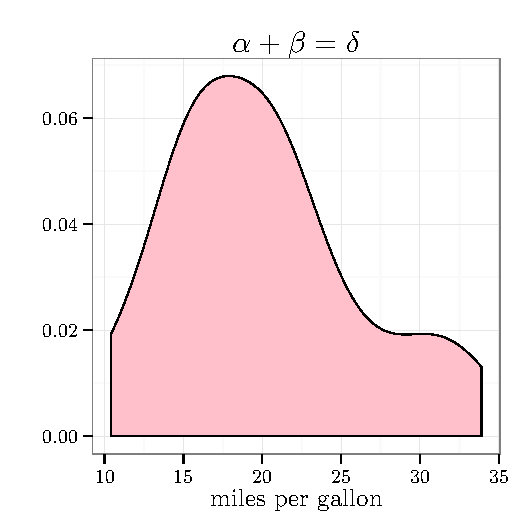
\includegraphics[width=0.5\textwidth]{figure/GraphShow-1} 

}



\end{knitrout}
\caption{This is where you explain your graph \label{graphDude}}
\end{figure}

\clearpage

\section{Git Stuff}

When working with OSX, one may want to change \texttt{engine = `sh'} to \texttt{engine = `bash'}.

\begin{knitrout}
\definecolor{shadecolor}{rgb}{0.969, 0.969, 0.969}\color{fgcolor}\begin{kframe}
\begin{GIT}\label{GITlabel}\hfill{}\begin{alltt}
git config --list
\end{alltt}

\begin{verbatim}
core.repositoryformatversion=0
core.filemode=true
core.bare=false
core.logallrefupdates=true
remote.origin.url=https://github.com/STAT-ATA-ASU/Tu-Huy.git
remote.origin.fetch=+refs/heads/*:refs/remotes/origin/*
branch.master.remote=origin
branch.master.merge=refs/heads/master
\end{verbatim}
\end{GIT}\end{kframe}
\end{knitrout}

Look at \textbf{R Code} \vref{test-a} to add $1 + 1$ and get the answer 2. The output from \textbf{Git Example} \vref{GITlabel} shows how my machine is configured. \textbf{Git Example} \vref{gitlog} shows the log.

\begin{knitrout}
\definecolor{shadecolor}{rgb}{0.969, 0.969, 0.969}\color{fgcolor}\begin{kframe}
\begin{GIT}\label{gitlog}\hfill{}\begin{alltt}
git log --pretty=oneline -3
\end{alltt}

\begin{verbatim}
4f0f4117400b2486dbb63146a3368211642351ff Commit
34cb1d5bda177368881d0e6db0fc01d8afb84326 YES
dafce642ce4f437816d401b7ba3fa2ad3a9f29c3 !!!
\end{verbatim}
\end{GIT}\end{kframe}
\end{knitrout}

\clearpage

\section{Using \LaTeX{} in Graphs}

How about some more \LaTeX{} in a \texttt{ggplot2} graph.

\begin{knitrout}
\definecolor{shadecolor}{rgb}{0.969, 0.969, 0.969}\color{fgcolor}\begin{kframe}
\begin{rcode}\label{molatex}\hfill{}\begin{alltt}
\hlstd{f} \hlkwb{<-} \hlkwa{function}\hlstd{(}\hlkwc{x}\hlstd{)\{}\hlkwd{sqrt}\hlstd{(}\hlnum{2}\hlopt{/}\hlstd{(x} \hlopt{-} \hlnum{1}\hlstd{))}\hlopt{*}\hlkwd{gamma}\hlstd{(x}\hlopt{/}\hlnum{2}\hlstd{)}\hlopt{/}\hlkwd{gamma}\hlstd{((x} \hlopt{-} \hlnum{1}\hlstd{)}\hlopt{/}\hlnum{2}\hlstd{)\}}
\hlkwd{library}\hlstd{(ggplot2)}
\hlstd{p} \hlkwb{<-} \hlkwd{ggplot}\hlstd{(}\hlkwd{data.frame}\hlstd{(}\hlkwc{x} \hlstd{=} \hlkwd{c}\hlstd{(}\hlnum{2}\hlstd{,} \hlnum{50}\hlstd{)),} \hlkwd{aes}\hlstd{(}\hlkwc{x} \hlstd{= x))}
\hlstd{p} \hlopt{+} \hlkwd{stat_function}\hlstd{(}\hlkwc{fun} \hlstd{= f)} \hlopt{+}
  \hlkwd{labs}\hlstd{(}\hlkwc{x} \hlstd{=} \hlstr{"$n$"}\hlstd{,} \hlkwc{y} \hlstd{=} \hlstr{"$\textbackslash{}\textbackslash{}frac\{\textbackslash{}\textbackslash{}sqrt\{2\}\textbackslash{}\textbackslash{}Gamma\textbackslash{}\textbackslash{}left(\textbackslash{}\textbackslash{}frac\{n\}\{2\}\textbackslash{}\textbackslash{}right)\}
       \{\textbackslash{}\textbackslash{}sqrt\{n-1\}\textbackslash{}\textbackslash{}Gamma\textbackslash{}\textbackslash{}left(\textbackslash{}\textbackslash{}frac\{n-1\}\{2\}\textbackslash{}\textbackslash{}right)\}$\textbackslash{}n"}\hlstd{)} \hlopt{+}
  \hlkwd{theme_bw}\hlstd{()} \hlopt{+}
  \hlkwd{geom_hline}\hlstd{(}\hlkwc{yintercept} \hlstd{=} \hlnum{1}\hlstd{,} \hlkwc{lty} \hlstd{=} \hlstr{"dashed"}\hlstd{)}
\end{alltt}
\end{rcode}\end{kframe}
\end{knitrout}

\begin{knitrout}
\definecolor{shadecolor}{rgb}{0.969, 0.969, 0.969}\color{fgcolor}

{\centering 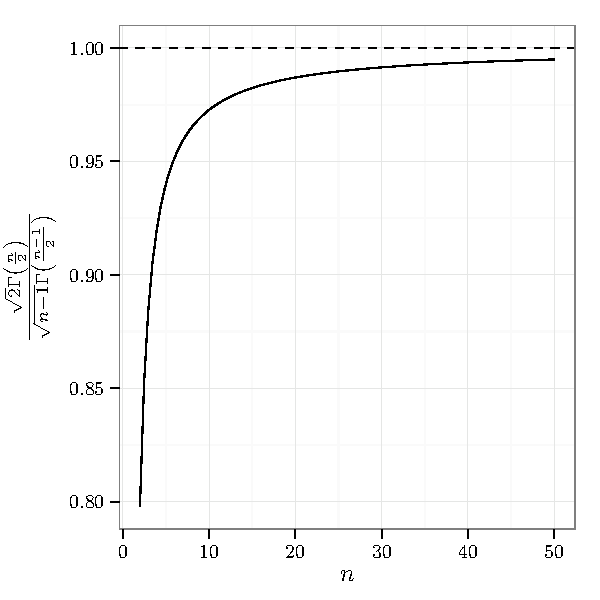
\includegraphics[width=1.0\textwidth]{figure/molatexFIG-1} 

}



\end{knitrout}

\begin{knitrout}
\definecolor{shadecolor}{rgb}{0.969, 0.969, 0.969}\color{fgcolor}

{\centering 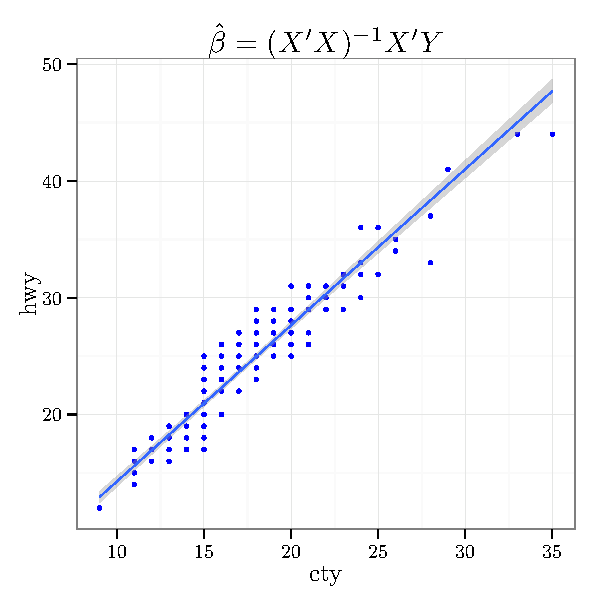
\includegraphics[width=\maxwidth]{figure/base-1} 

}



\end{knitrout}

\begin{itemize}\raggedright
  \item R version 3.2.2 (2015-08-14), \verb|x86_64-pc-linux-gnu|
  \item Locale: \verb|LC_CTYPE=en_US.UTF-8|, \verb|LC_NUMERIC=C|, \verb|LC_TIME=en_US.UTF-8|, \verb|LC_COLLATE=en_US.UTF-8|, \verb|LC_MONETARY=en_US.UTF-8|, \verb|LC_MESSAGES=en_US.UTF-8|, \verb|LC_PAPER=en_US.UTF-8|, \verb|LC_NAME=C|, \verb|LC_ADDRESS=C|, \verb|LC_TELEPHONE=C|, \verb|LC_MEASUREMENT=en_US.UTF-8|, \verb|LC_IDENTIFICATION=C|
  \item Base packages: base, datasets, graphics, grDevices,
    methods, stats, utils
  \item Other packages: ggplot2~1.0.1, knitr~1.11,
    tikzDevice~0.8.1
  \item Loaded via a namespace (and not attached):
    codetools~0.2-14, colorspace~1.2-6, digest~0.6.8,
    evaluate~0.7.2, filehash~2.3, formatR~1.2.1, grid~3.2.2,
    gtable~0.1.2, highr~0.5.1, labeling~0.3, magrittr~1.5,
    MASS~7.3-44, munsell~0.4.2, plyr~1.8.3, proto~0.3-10,
    Rcpp~0.12.1, reshape2~1.4.1, scales~0.3.0, stringi~1.0-1,
    stringr~1.0.0, tools~3.2.2
\end{itemize}




\end{document}
